\documentclass[12pt] {article}
\usepackage{times}
\usepackage[margin=1in,bottom=1in,top=0.5in]{geometry}

\usepackage{hhline}
\usepackage{subfig}
\usepackage{amsmath}
\usepackage{amsfonts}
\usepackage[inline,shortlabels]{enumitem}%enumerate with letters
\usepackage{mathrsfs} 
\usepackage[square,numbers]{natbib}
\usepackage{graphicx}
\usepackage{natbib}


\begin{document}
\bibliographystyle{apalike}
\title{
\begin{Large}
ECS 277 - Winter 2019 - Final Project Proposal\\\vspace{3.0mm}
\end{Large}
Ambient Occlusion for Iso-surfaces Visualization
}
\author{Ahmed Mahmoud}
\date{}
\maketitle

%============Table========
%\begin{figure}[tbh]
% \centering    
%\begin{tabular}{ |p{4cm}|| p{2cm}|p{2cm}|p{2cm}|p{2cm}|}
% \hline
% & Processor 1 &  Processor 2  & Processor 3 & Processor 4\\ \hhline{|=|=|=|=|=|}
% \hline
% Performance          &$1.08$        &$1.425$       &\textbf{1.52}  &   \\
% \hline
%\end{tabular} 
%\caption{Metric table for the four processors}
%   \label{tab:metric}
%\end{figure} 
%============Figure========
%\begin{figure}[!tbh]
%\centering        
%   \subfloat {\includegraphics[width=0.65\textwidth]{fig2_4.png}}
%   \caption{ }
%   \label{fig:fig}
%\end{figure}

%\begin{enumerate}[(a)]
%\end{enumerate}

\section*{Abstract}
\paragraph{Iso-surface.} In volumetric data visualization, the user might be interested in visualization certain iso-surfaces; surface where the density function is constant. For instance, examining the hard tissues (e.g., tooth, bones) in CT or MRI scans on structured grid. Extracting iso-surface can be done using Marching Cube. Efficient data-structure can be used to accelerate such extraction specially for dynamically changing iso-surface (e.g., numerical simulation solutions). Among several, Volumetric Dynamic Grid (VDB)~\citep{museth2013vdb} is one of the most successful for representing dynamic sparse volume data. VDB supports arbitrary grid topology, hierarchical signed distance flood-filling, and adaptive sampling.

\paragraph{Ambient Occlusion.} Global illumination (GI) can be used to improve the visual appearance of iso-surfaces %(Figure~\ref{fig:ao}). 
GI can be done via ray-tracing which is computationally expensive and can be the bottleneck for topology-changing applications when interactive rate is desired. In this project, we choose to implement the ambient occlusion for the iso-surfaces. Ambient occlusion simulates the shadowing caused by objects blocking the ambient light and can improve the visual appearance of the iso-surface greatly. Since ambient occlusion does not depend on the light direction but on the surface topology, it can be pre-computed and stored statically. However, for topology-changing situations, pre-computation is not feasible anymore. Thus, we aim into using the efficient representation of the volume data by VDB to also enhance the visual appearance of the extracted iso-surface. 
\\

%\begin{figure}[!tbh]
%\centering        
%   \subfloat [Local Illumination] {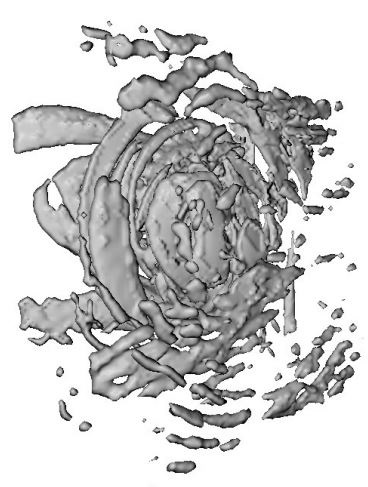
\includegraphics[width=0.3\textwidth]{local.JPG}}
%   \subfloat [Ambient Occlusion]{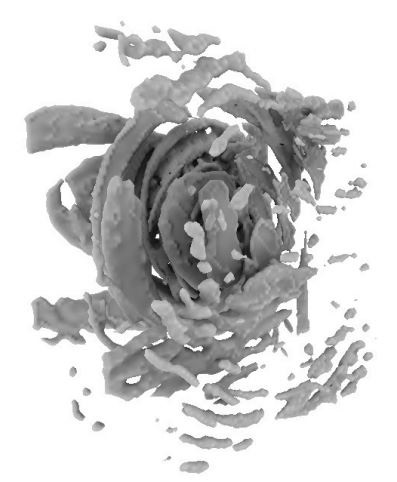
\includegraphics[width=0.3\textwidth]{AO.JPG}}
%   \caption{Ambient occlusion can enhance the realism of volume rendering (image source~\citep{singh2009fast}). }
%   \label{fig:ao}
%\end{figure}


\noindent In this project, we propose a new technique to simulate the ambient occlusion. Using VDB data-structure, a narrow-band (of voxels) can be construct very quickly around the desired iso-surface. To collect the neighbor information for ambient occlusion calculation, we can use flood-fill technique to propagate the sign-distance from which ambient occlusion can be approximated. 


\bibliography{mybib}
\end{document}